% !TeX program = xelatex
\documentclass[UTF8,12pt,a4paper]{ctexart}
\usepackage{amsmath,amssymb}
\usepackage{geometry}
\usepackage{tikz}
\geometry{margin=2cm}

% ===== 水印设置 =====
\usepackage{xcolor}
\usepackage{eso-pic}
\usepackage{graphicx}

\newcommand{\WMText}{贺昱超学习资料}
\newcommand{\WMScale}{2.28}
\newcommand{\WMAngle}{45}
\colorlet{WMColor}{black!8}

\AddToShipoutPictureBG{%
  \AtPageLowerLeft{%
    \put(\LenToUnit{0.66\paperwidth},\LenToUnit{0.70\paperheight}){%
      \rotatebox{\WMAngle}{\scalebox{\WMScale}{\textcolor{WMColor}{\WMText}}}%
    }%
    \put(\LenToUnit{0.33\paperwidth},\LenToUnit{0.50\paperheight}){%
      \rotatebox{\WMAngle}{\scalebox{\WMScale}{\textcolor{WMColor}{\WMText}}}%
    }%
    \put(\LenToUnit{0.66\paperwidth},\LenToUnit{0.30\paperheight}){%
      \rotatebox{\WMAngle}{\scalebox{\WMScale}{\textcolor{WMColor}{\WMText}}}%
    }%
  }%
}

\begin{document}

% ===== 试卷页眉 =====
\begin{center}
{\LARGE \textbf{贺昱琪阶第一段练习卷}} \\
\vspace{0.6cm}

\vspace{0.4cm}
\hrule
\end{center}
\vspace{0.5cm}

% ===== 试卷内容 =====
\section*{一、简便计算（每题 10 分，共 10 分）}
\vspace{0.3cm}

\noindent \textbf{1.} 计算：$\displaystyle \frac{2024 + \dfrac{1}{2023}}{2023 + \dfrac{1}{2024}} - \frac{2022 + \dfrac{1}{2023}}{2023 + \dfrac{1}{2022}}$
\vspace{2.5cm}

\section*{二、解方程组（每题 10 分，共 20 分）}
\vspace{0.3cm}

\noindent \textbf{2.} 解下列二元一次方程组：
\[
\begin{cases} 
2x - y = 3 \\ 
\dfrac{x-1}{2} = \dfrac{y-3}{3} 
\end{cases}
\]
\vspace{3.5cm}

\noindent \textbf{3.} 解下列二元一次方程组：
\[
\begin{cases} 
4x - y = 7 \\ 
\dfrac{x+1}{2} = \dfrac{y-1}{2} 
\end{cases}
\]
\vspace{3.5cm}


\section*{三、填空题（每题 10 分，共 20 分）}
\vspace{0.3cm}

\noindent \textbf{4.} 
\begin{minipage}[t]{0.70\textwidth}
在长方形 ABCD 中，已知两邻边 $AD=24$，$AB=10$，对角线 $AC=26$，$O$ 为对角线交点。$P$ 是 $AD$ 边上异于 $A$ 和 $D$ 的一个动点，过点 $P$ 分别向 $OA, OD$ 作垂线 $PE, PF$，那么 $PE+PF$ 有\underline{\hspace{3em}}值（填“最大”、“最小”或“定”），这个值为\underline{\hspace{3em}}。
\end{minipage}
\hfill
\begin{minipage}[t]{0.25\textwidth}
\vspace{-0.5cm}
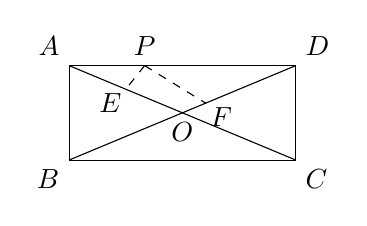
\begin{tikzpicture}[scale=0.12]
\draw (0,0) node[below left]{$B$} -- (24,0) node[below right]{$C$} -- (24,10) node[above right]{$D$} -- (0,10) node[above left]{$A$} -- cycle;
\draw (0,10) -- (24,0); \draw (0,0) -- (24,10);
\node[below] at (12,5) {$O$};
\coordinate (P) at (8,10); \node[above] at (P) {$P$};
\draw[dashed] (P) -- (6, 7.5) node[below left=-2pt]{$E$};
\draw[dashed] (P) -- (14.5, 6.0) node[below right=-2pt]{$F$};
\end{tikzpicture}
\end{minipage}

\vspace{1.5cm}

\noindent \textbf{5.} 老师在黑板上写了若干个从 1 开始的连续自然数：$1, 2, 3, 4, \dots$，后来擦掉其中的一个，剩下的数的平均数是 $22\dfrac{8}{21}$，擦掉的自然数是\underline{\hspace{3em}}。

\vspace{0.5cm}
\newpage

\section*{四、解决问题（每题 20 分，共 60 分）}
\vspace{0.5cm}

\noindent \textbf{6.} 快、慢两车同时从甲、乙两地相向开出，快车行完全程需 12 小时，慢车行完全程需 20 小时。两车在途中相遇后，快车又行了 110 千米，这时快车已行了全程的 $\dfrac{9}{10}$。甲、乙两地相距多少千米？
\vspace{7cm}

\noindent \textbf{7.} 一列火车出发 2.5 小时后因故停车 0.5 小时，然后以原速的 $\dfrac{3}{4}$ 前进，最终到达目的地晚 1.5 小时。若出发 2.5 小时后又前进 120 公里再因故停车 0.5 小时，然后同样以原速的 $\dfrac{3}{4}$ 前进，则到达目的地仅晚 1 小时。那么整个路程为多少公里？
\vspace{7cm}

\newpage
\noindent \textbf{8.} 将长方体石块（长$a$、宽$b$、高$c$，且 $a>b>c$）放入一圆柱形水槽内，并向水槽内匀速注水，速度为 $v \text{ cm}^3/\text{s}$，直至注满水槽为止。石块可以以三种不同的方式完全放入水槽内，如图1~图3所示。在这三种情况下，水槽内的水深 $h$ (cm) 与注水时间 $t$ (s) 的函数关系如图4~图6所示。

\vspace{0.5cm}
\begin{center}
\begin{tikzpicture}[scale=0.28]
  \draw (0,4) ellipse (3 and 0.8); \draw (-3,0) -- (-3,4); \draw (3,0) -- (3,4);
  \draw (-3,0) arc (180:360:3 and 0.8); \draw[dashed] (3,0) arc (0:180:3 and 0.8);
  \draw[fill=gray!30] (-1.5, -0.4) rectangle (1.5, 0.6); \draw[fill=gray!50] (1.5, -0.4) -- (2.2, 0) -- (2.2, 1) -- (1.5, 0.6) -- cycle; \draw[fill=gray!20] (-1.5, 0.6) -- (1.5, 0.6) -- (2.2, 1) -- (-0.8, 1) -- cycle; \node[below] at (0,-1.5) {图1};
\end{tikzpicture}
\hspace{0.5cm}
\begin{tikzpicture}[scale=0.28]
  \draw (0,4) ellipse (3 and 0.8); \draw (-3,0) -- (-3,4); \draw (3,0) -- (3,4);
  \draw (-3,0) arc (180:360:3 and 0.8); \draw[dashed] (3,0) arc (0:180:3 and 0.8);
  \draw[fill=gray!30] (-0.8, -0.6) rectangle (0.8, 3.5); \draw[fill=gray!50] (0.8, -0.6) -- (1.5, -0.2) -- (1.5, 3.9) -- (0.8, 3.5) -- cycle; \draw[fill=gray!20] (-0.8, 3.5) -- (0.8, 3.5) -- (1.5, 3.9) -- (-0.1, 3.9) -- cycle; \node[below] at (0,-1.5) {图2};
\end{tikzpicture}
\hspace{0.5cm}
\begin{tikzpicture}[scale=0.28]
  \draw (0,4) ellipse (3 and 0.8); \draw (-3,0) -- (-3,4); \draw (3,0) -- (3,4);
  \draw (-3,0) arc (180:360:3 and 0.8); \draw[dashed] (3,0) arc (0:180:3 and 0.8);
  \draw[fill=gray!30] (-1, -0.5) rectangle (1, 2.5); \draw[fill=gray!50] (1, -0.5) -- (1.8, -0.1) -- (1.8, 2.9) -- (1, 2.5) -- cycle; \draw[fill=gray!20] (-1, 2.5) -- (1, 2.5) -- (1.8, 2.9) -- (-0.2, 2.9) -- cycle; \node[below] at (0,-1.5) {图3};
\end{tikzpicture}
\end{center}

\vspace{0.5cm}
\begin{center}
\begin{tikzpicture}[scale=0.65]
  \draw[->] (-0.2,0) -- (3.5,0) node[right]{\scriptsize $t/\text{s}$}; \draw[->] (0,-0.2) -- (0,3) node[above]{\scriptsize $h/\text{cm}$}; \draw (0,0) node[below left]{\scriptsize $O$};
  \draw[thick] (0,0) -- (1.5, 1.2) node[above left=-2pt]{\scriptsize $A$} -- (2.8, 2.5) node[above]{\scriptsize $B$};
  \draw[dashed] (1.5,0) node[below]{\scriptsize 45} -- (1.5,1.2) -- (0,1.2) node[left]{\scriptsize 10};
  \draw[dashed] (2.8,0) node[below]{\scriptsize 165} -- (2.8,2.5) -- (0,2.5) node[left]{\scriptsize 20}; \node[below] at (1.5,-0.8) {图4};
\end{tikzpicture}
\hspace{0.5cm}
\begin{tikzpicture}[scale=0.65]
  \draw[->] (-0.2,0) -- (3.5,0) node[right]{\scriptsize $t/\text{s}$}; \draw[->] (0,-0.2) -- (0,3) node[above]{\scriptsize $h/\text{cm}$}; \draw (0,0) node[below left]{\scriptsize $O$};
  \draw[thick] (0,0) -- (2.2, 2.0) node[above left=-2pt]{\scriptsize $C$} -- (2.8, 2.5) node[above]{\scriptsize $D$};
  \draw[dashed] (2.2,0) node[below]{\scriptsize 105} -- (2.2,2.0) -- (0,2.0) node[left]{\scriptsize 15};
  \draw[dashed] (2.8,0) node[below]{\scriptsize 165} -- (2.8,2.5) -- (0,2.5) node[left]{\scriptsize 20}; \node[below] at (1.5,-0.8) {图5};
\end{tikzpicture}
\hspace{0.5cm}
\begin{tikzpicture}[scale=0.65]
  \draw[->] (-0.2,0) -- (3.5,0) node[right]{\scriptsize $t/\text{s}$}; \draw[->] (0,-0.2) -- (0,3) node[above]{\scriptsize $h/\text{cm}$}; \draw (0,0) node[below left]{\scriptsize $O$};
  \draw[thick] (0,0) -- (2.8, 2.5) node[above]{\scriptsize $E$};
  \draw[dashed] (2.8,0) node[below]{\scriptsize 165} -- (2.8,2.5) -- (0,2.5) node[left]{\scriptsize 20}; \node[below] at (1.5,-0.8) {图6};
\end{tikzpicture}
\end{center}
\vspace{0.3cm}

\noindent (1) 请分别将三种放置方式的示意图和与之对应的关系图象用线连接起来（直接在上方图中连线或写出对应关系即可）；\\
(2) 水槽的高\underline{\hspace{3em}}cm；石块的长 $a=$\underline{\hspace{3em}}cm；宽 $b=$\underline{\hspace{3em}}cm；高 $c=$\underline{\hspace{3em}}cm；\\
(3) 求圆柱形水槽的底面积 $S$（用含 $v$ 的式子表示），并写出完整的计算过程。

\newpage
% ===== 五、 附加提升题 =====
\section*{五、附加提升题}
\vspace{0.5cm}

\noindent \textbf{9.} \begin{minipage}[t]{0.65\textwidth}
利用两块长方体木块测量一张桌子的高度。首先按图①方式放置，再交换两木块的位置，按图②方式放置。测量的数据如图，则桌子的高度是\underline{\hspace{3em}}cm。
\end{minipage}
\hfill
\begin{minipage}[t]{0.30\textwidth}
\vspace{-0.8cm}
\begin{tikzpicture}[scale=0.3]
  % Setup 1
  \draw[thick] (0,0) -- (0,3) -- (3,3) -- (3,0);
  \draw[thick] (0.5,0) -- (0.5,2.5) -- (2.5,2.5) -- (2.5,0);
  \draw[fill=gray!80] (2,3) rectangle (2.8,4.5);
  \draw[fill=gray!80] (3,0) rectangle (4.5,0.8);
  \draw[<->] (5.2, 0.8) -- (5.2, 4.5) node[midway, right] {\scriptsize 80cm};
  \draw[dashed] (2.8,4.5) -- (5.2,4.5);
  \draw[dashed] (4.5,0.8) -- (5.2,0.8);
  \node at (1.5, -1) {①};
  % Setup 2
  \begin{scope}[shift={(8,0)}]
  \draw[thick] (0,0) -- (0,3) -- (3,3) -- (3,0);
  \draw[thick] (0.5,0) -- (0.5,2.5) -- (2.5,2.5) -- (2.5,0);
  \draw[fill=gray!80] (1.5,3) rectangle (3,3.8);
  \draw[fill=gray!80] (3,0) rectangle (3.8,1.5);
  \draw[<->] (4.6, 1.5) -- (4.6, 3.8) node[midway, right] {\scriptsize 70cm};
  \draw[dashed] (3,3.8) -- (4.6,3.8);
  \draw[dashed] (3.8,1.5) -- (4.6,1.5);
  \node at (1.5, -1) {②};
  \end{scope}
\end{tikzpicture}
\end{minipage}
\vspace{1cm}

\noindent \textbf{10.} 已知等腰三角形一腰上的高和另一腰的夹角是 $25^\circ$，则这个等腰三角形的底角度数为\underline{\hspace{3em}}。
\vspace{1.5cm}

\noindent \textbf{11.} \begin{minipage}[t]{0.70\textwidth}
如图，“回”字形的道路宽为 1 米，整个“回”字形是一个长 16 米，宽 8 米的长方形场地。如果小丽沿着小路的中间从内部出发走完这条小路，那么她共走\underline{\hspace{3em}}米。
\end{minipage}
\hfill
\begin{minipage}[t]{0.25\textwidth}
\vspace{-0.5cm}
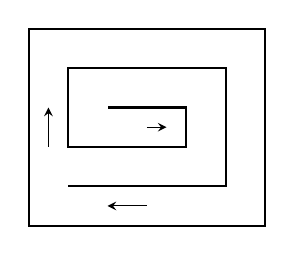
\begin{tikzpicture}[scale=0.25]
  \draw[thick] (0,0) rectangle (12,10);
  \draw[thick] (2,2) -- (10,2) -- (10,8) -- (2,8) -- (2,4) -- (8,4) -- (8,6) -- (4,6);
  \draw[->, >=stealth] (6,5) -- (7,5);
  \draw[->, >=stealth] (1,4) -- (1,6);
  \draw[->, >=stealth] (6,1) -- (4,1);
\end{tikzpicture}
\end{minipage}
\vspace{1.5cm}

\noindent \textbf{12.} 单独完成一项任务，甲按规定时间可提前 2 天完成，乙则要超过规定时间 3 天才能完成。如果甲、乙二人合作 2 天后，剩下的由乙单独做，那么刚好在规定时间完成。问：甲、乙二人合作需多少天完成该任务？
\vspace{4.5cm}

\noindent \textbf{13.} 快、慢两车同时从甲、乙两地相向开出，快车行完全程需 10 小时，慢车行完全程需 15 小时。两车在途中相遇后，快车又行了 96 千米，这时快车已行了全程的 $\dfrac{4}{5}$。甲乙两地相距多少千米？
\vspace{4.5cm}

\newpage
\noindent \textbf{14.} 将长方体石块（长$a$、宽$b$、高$c$，且 $a>b>c$）放入一圆柱形水槽内，并向水槽内匀速注水，速度为 $v \text{ cm}^3/\text{s}$，直至注满水槽为止。石块可以以三种不同的方式完全放入水槽内。在这三种情况下，水槽内的水深 $h$ (cm) 与注水时间 $t$ (s) 的函数关系如图4~图6所示。

\vspace{0.5cm}
\begin{center}
\begin{tikzpicture}[scale=0.28]
  \draw (0,4) ellipse (3 and 0.8); \draw (-3,0) -- (-3,4); \draw (3,0) -- (3,4);
  \draw (-3,0) arc (180:360:3 and 0.8); \draw[dashed] (3,0) arc (0:180:3 and 0.8);
  \draw[fill=gray!30] (-1.5, -0.4) rectangle (1.5, 0.6); \draw[fill=gray!50] (1.5, -0.4) -- (2.2, 0) -- (2.2, 1) -- (1.5, 0.6) -- cycle; \draw[fill=gray!20] (-1.5, 0.6) -- (1.5, 0.6) -- (2.2, 1) -- (-0.8, 1) -- cycle; \node[below] at (0,-1.5) {图1};
  \node at (0, 0.1) {$c$}; \node at (1.85, 0.3) {$b$}; \node at (0, -0.6) {$a$};
\end{tikzpicture}
\hspace{0.5cm}
\begin{tikzpicture}[scale=0.28]
  \draw (0,4) ellipse (3 and 0.8); \draw (-3,0) -- (-3,4); \draw (3,0) -- (3,4);
  \draw (-3,0) arc (180:360:3 and 0.8); \draw[dashed] (3,0) arc (0:180:3 and 0.8);
  \draw[fill=gray!30] (-0.8, -0.6) rectangle (0.8, 3.5); \draw[fill=gray!50] (0.8, -0.6) -- (1.5, -0.2) -- (1.5, 3.9) -- (0.8, 3.5) -- cycle; \draw[fill=gray!20] (-0.8, 3.5) -- (0.8, 3.5) -- (1.5, 3.9) -- (-0.1, 3.9) -- cycle; \node[below] at (0,-1.5) {图2};
  \node at (0, 1.5) {$a$}; \node at (1.15, -0.4) {$c$}; \node at (1.5, 1.85) {$b$};
\end{tikzpicture}
\hspace{0.5cm}
\begin{tikzpicture}[scale=0.28]
  \draw (0,4) ellipse (3 and 0.8); \draw (-3,0) -- (-3,4); \draw (3,0) -- (3,4);
  \draw (-3,0) arc (180:360:3 and 0.8); \draw[dashed] (3,0) arc (0:180:3 and 0.8);
  \draw[fill=gray!30] (-1, -0.5) rectangle (1, 2.5); \draw[fill=gray!50] (1, -0.5) -- (1.8, -0.1) -- (1.8, 2.9) -- (1, 2.5) -- cycle; \draw[fill=gray!20] (-1, 2.5) -- (1, 2.5) -- (1.8, 2.9) -- (-0.2, 2.9) -- cycle; \node[below] at (0,-1.5) {图3};
  \node at (0, 1) {$b$}; \node at (1.4, -0.3) {$c$}; \node at (1.8, 1.4) {$a$};
\end{tikzpicture}
\end{center}

\vspace{0.5cm}
\begin{center}
\begin{tikzpicture}[scale=0.65]
  \draw[->] (-0.2,0) -- (3.5,0) node[right]{\scriptsize $t/\text{s}$}; \draw[->] (0,-0.2) -- (0,3) node[above]{\scriptsize $h/\text{cm}$}; \draw (0,0) node[below left]{\scriptsize $O$};
  \draw[thick] (0,0) -- (1.5, 1.2) node[above left=-2pt]{\scriptsize $A$} -- (2.8, 2.5) node[above]{\scriptsize $B$};
  \draw[dashed] (1.5,0) node[below]{\scriptsize 21} -- (1.5,1.2) -- (0,1.2) node[left]{\scriptsize 6};
  \draw[dashed] (2.8,0) node[below]{\scriptsize 53} -- (2.8,2.5) -- (0,2.5) node[left]{\scriptsize 10}; \node[below] at (1.5,-0.8) {图4};
\end{tikzpicture}
\hspace{0.5cm}
\begin{tikzpicture}[scale=0.65]
  \draw[->] (-0.2,0) -- (3.5,0) node[right]{\scriptsize $t/\text{s}$}; \draw[->] (0,-0.2) -- (0,3) node[above]{\scriptsize $h/\text{cm}$}; \draw (0,0) node[below left]{\scriptsize $O$};
  \draw[thick] (0,0) -- (2.2, 2.0) node[above left=-2pt]{\scriptsize $C$} -- (2.8, 2.5) node[above]{\scriptsize $D$};
  \draw[dashed] (2.2,0) node[below]{\scriptsize 45} -- (2.2,2.0) -- (0,2.0) node[left]{\scriptsize 9};
  \draw[dashed] (2.8,0) node[below]{\scriptsize 53} -- (2.8,2.5) -- (0,2.5) node[left]{\scriptsize 10}; \node[below] at (1.5,-0.8) {图5};
\end{tikzpicture}
\hspace{0.5cm}
\begin{tikzpicture}[scale=0.65]
  \draw[->] (-0.2,0) -- (3.5,0) node[right]{\scriptsize $t/\text{s}$}; \draw[->] (0,-0.2) -- (0,3) node[above]{\scriptsize $h/\text{cm}$}; \draw (0,0) node[below left]{\scriptsize $O$};
  \draw[thick] (0,0) -- (2.8, 2.5) node[above]{\scriptsize $E$};
  \draw[dashed] (2.8,0) node[below]{\scriptsize 53} -- (2.8,2.5) -- (0,2.5) node[left]{\scriptsize 10}; \node[below] at (1.5,-0.8) {图6};
\end{tikzpicture}
\end{center}
\vspace{0.3cm}

\noindent (1) 请分别将三种放置方式的示意图和与之对应的关系图象用线连接起来（直接在图中连线或写出对应关系即可）；\\
(2) 水槽的高\underline{\hspace{3em}}cm；石块的长 $a=$\underline{\hspace{3em}}cm；宽 $b=$\underline{\hspace{3em}}cm；高 $c=$\underline{\hspace{3em}}cm；\\
(3) 求圆柱形水槽的底面积 $S$，并写出计算过程。


\end{document}